\problemset{Комбинаторика и теория графов}
\problemset{Индивидуальное домашнее задание №1}	% поменяйте номер ИДЗ

\renewcommand*{\proofname}{Решение}

%%%%%%%%%%%%%% ЗАДАНИЕ №1 %%%%%%%%%%%%%%
%% Условие задания №1
\begin{problem}[1]
	Бинарное отношение задано матрицей. С помощьюалгоритма Уоршелла найдиет его транзитивное замыкание.
    \par

    \[\begin{pmatrix}
        0 & 0 & 0 & 0 & 0\\
        1 & 0 & 1 & 1 & 0\\
        0 & 0 & 0 & 1 & 1\\
        0 & 0 & 1 & 1 & 0\\
        1 & 1 & 0 & 1 & 1
    \end{pmatrix}\]
    
\end{problem}

%% Решение задания №1
\begin{proof}

    \begin{figure}[h]
     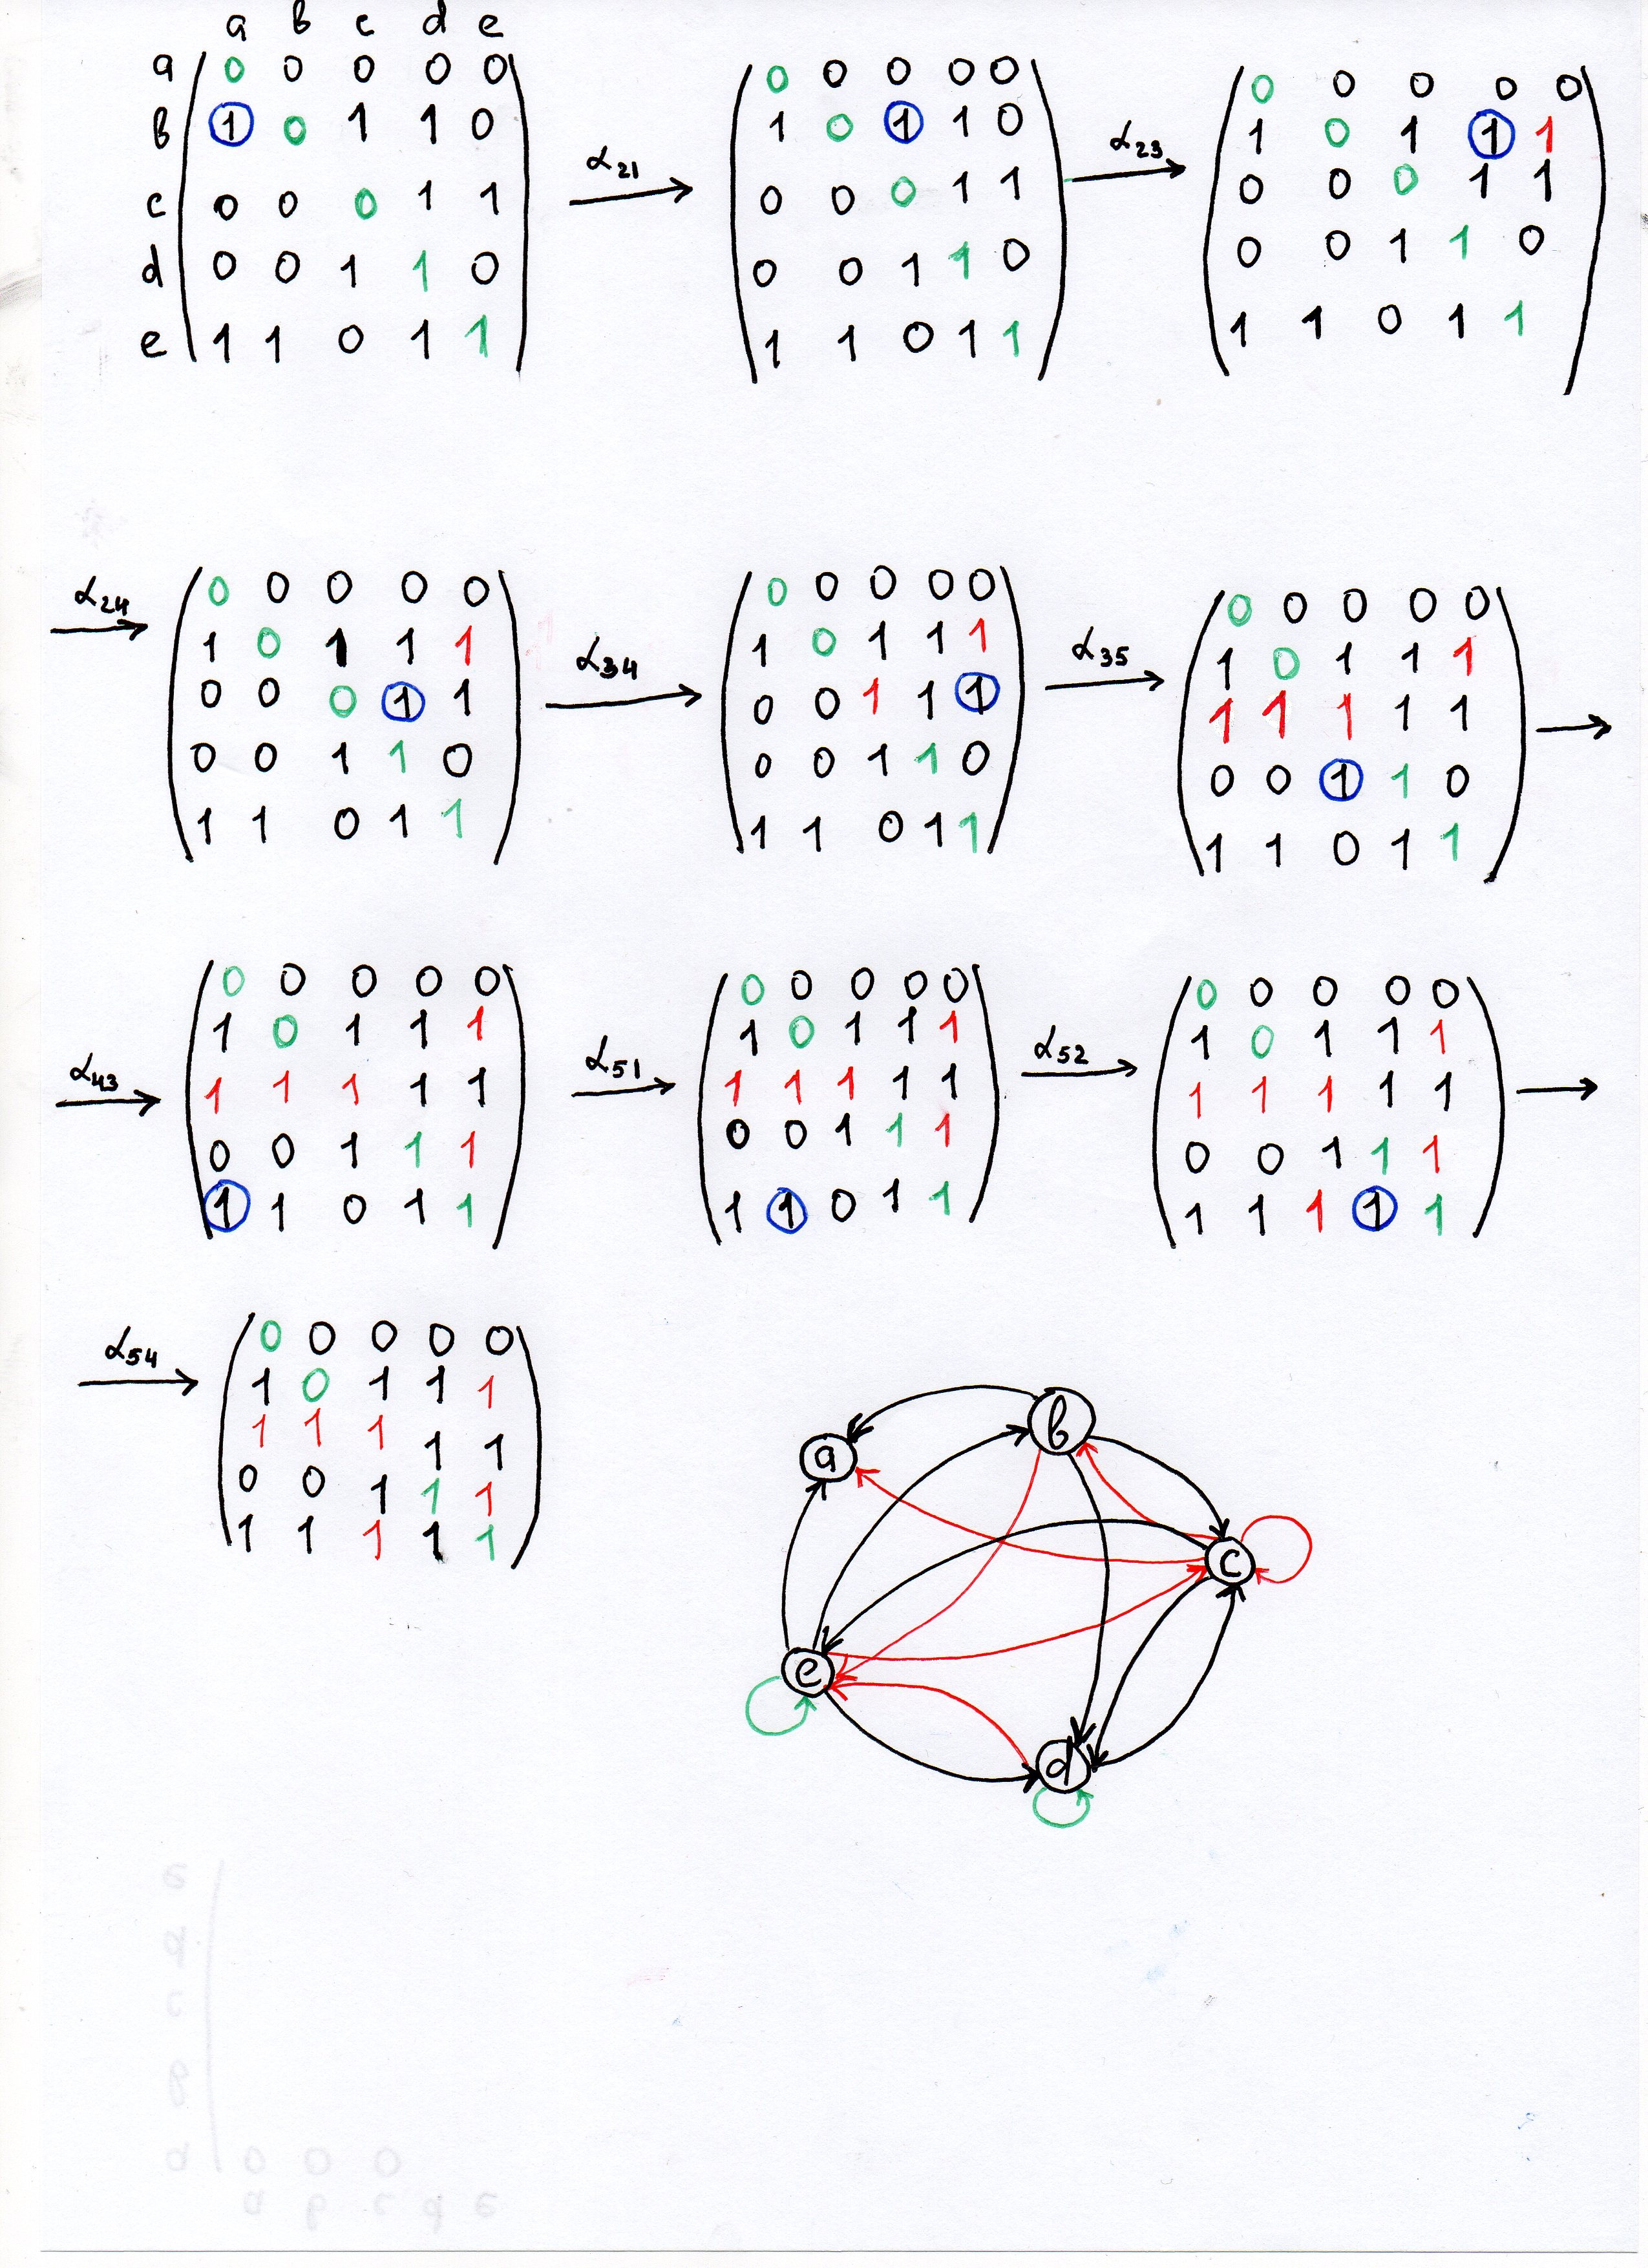
\includegraphics[width=0.634\linewidth]{pics/1thsolution.jpg}
     \label{fig:dm}
    \end{figure}

 Зелёным цветом обозначаются элементы, принадлежащие главной диагонали булевой матрицы. Синим цветом обозначается, текущая рассматриваемая единица. У нее есть номер в виде $\alpha_{ij}$, где i - это номер строки, а j - столбца. Таким образом, я обозначаю текущее состояние матрицы, после проделанного дизьюнктивного объединения строчек (i-я строка объединяется с j-й).
 
\end{proof}

%%%%%%%%%%%%%% ЗАДАНИЕ №4 %%%%%%%%%%%%%%
%% Условие задания №4
\begin{problem}[4]
	а) Постройте код Прюфера, для данного дерева:
 
    \begin{figure}[h]
     \centering
     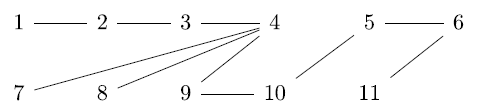
\includegraphics[width=0.5\linewidth]{pics/4thGraph.png}
     \label{fig:dm}
    \end{figure}

    б) Постройте дерево по коду Прюфера: 2 4 10 11 8 8 1 2 10.
\end{problem}

%% Решение задания №4
\begin{proof}
    а) Удаляем лист с наименьшим номером, и записываем вершину из которого он исходил. Последовательность должна быть длиной n - 2, где n - количество вершин дерева:
   
    Ответ: [2 3 4 4 4 9 10 5]

    б) Берём первое число a из кода Прюфера, затем находим в массиве вершин графа наименьший номер b, которого нет в коде. Затем записывае ребро a - b и удаляем их из соответствующих массивов.

    \begin{figure}[h]
     \centering
     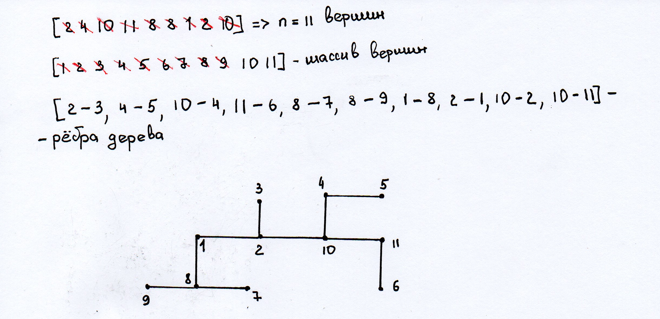
\includegraphics[width=0.7\linewidth]{pics/4thBsolution.png}
     \label{fig:dm}
    \end{figure}
    
\end{proof}

%%%%%%%%%%%%%% ЗАДАНИЕ №5 %%%%%%%%%%%%%%
%% Условие задания №5
\begin{problem}[5]
    Является ли граф: 
    \begin{figure}[h]
    \centering
     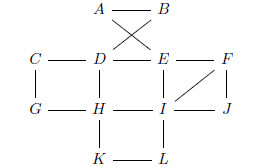
\includegraphics[width=0.4\linewidth]{pics/Graph5th.png}
     \label{fig:dm}
    \end{figure}
    
    б) гамильтоновым, полугамильтоновым?
    
    г) вершинно-двусвязным?

    д) рёберно-двусвязным?

    е) постройте дерево блоков и точек сочленения.
\end{problem}

%% Решение задания №5
\begin{proof}
	б) Граф гамильтонов, поскольку имеет гамильтонов цикл: BAEFJILKHGCD
    
    г) Граф является вершинно-двусвязным, поскольку удаление любой его 1-й вершины не ведёт к потере связности графа.

    д) Граф является рёберно двусвязным, поскольку он является вершинно-двусвязным.

    e) Поскольку граф вершинно-двусвязный, у него нет точек-сочленения, а дерево состоит из 1 блока, включающего все вершины.

    \begin{figure}[h]
    \centering
     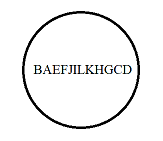
\includegraphics[width=0.2\linewidth]{pics/5thEsolution.png}
     \label{fig:dm}
    \end{figure}
    
\end{proof}

%%%%%%%%%%%%%% ЗАДАНИЕ №6 %%%%%%%%%%%%%%
%% Условие задания №6
\begin{problem}[6]
	При помощи графа де Брюина найдите все слова наименьшей длины, которые содержат подстроки FRC, RCF, FRO, FCO, OCF, CFR, CFC, ROC.
\end{problem}

%% Решение задания №6
\begin{proof}
    Составим граф де Брюина по данным подстрокам:

    \begin{figure}[h]
    \centering
     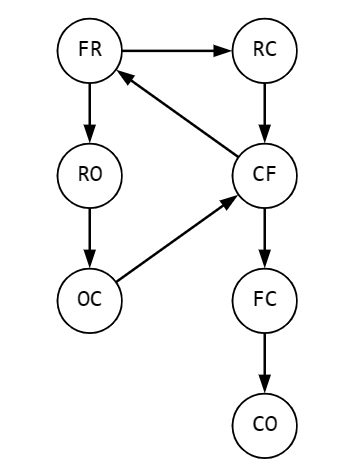
\includegraphics[width=0.35\linewidth]{pics/6thGraph.png}
     \label{fig:dm}
    \end{figure}

    Словом наименьшей длины является путь содержащий все префиксы и суффиксы подстрок, то есть нужно совершить Эйлеров обход графа де Брюина.
    
    Начало пути вершина FR:
    
    1) FRCFROCFCO
    
    2) FROCFRCFCO 
    
\end{proof}

%%%%%%%%%%%%%% ЗАДАНИЕ №7 %%%%%%%%%%%%%%
%% Условие задания №7
\begin{problem}[7]

	Найдите наибольшее возможное количество рёбер в двудольном плоском графе с 82 вершинами.
    
\end{problem}

%% Решение задания №7
\begin{proof}

    Для того, чтобы количество рёбер в двудольном графе было наибольшим -  количество вершин в каждой доле должно быть примерно равным. Так как у нас 82 вершины, то их можно разделить на 2 доли по 41 вершине. Тогда максимальное количество рёбер будет равным $41 * 41 = 1681$

\end{proof}

%%%%%%%%%%%%%% ЗАДАНИЕ №9 %%%%%%%%%%%%%%
%% Условие задания №9
\begin{problem}[9]

	Найдите радиус, диаметр и центр данного дерева:
    
    \centering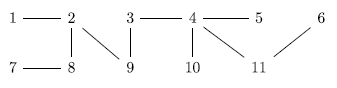
\includegraphics[width=0.6\linewidth]{pics/9thGraph.png}
    
\end{problem}

%% Решение задания №9
\begin{proof}

    Ищем путь с максимальной длиной из каждой вершины в остальные:

    (1 - 6) = 6

    (2 - 6) = 5

    (3 - 7) = 4

    (4 - 7) = 5

    (5 - 7) = 6

    (6 - 7) = 7

    (7 - 6) = 7

    (8 - 6) = 6

    (9 - 6) = 4

    (10 - 7) = 6

    (11 - 7) = 6

    Тогда \textbf{радиус} графа равен 4, \textbf{диаметр} равен 7, а \textbf{центром} могут быть вершины 3 или 9.

\end{proof}

%%%%%%%%%%%%%% ЗАДАНИЕ №10 %%%%%%%%%%%%%%
%% Условие задания №10
\begin{problem}[10]

	Найдите радиус, диаметр и центр данного графа:
    
    \centering\includegraphics[width=0.4\linewidth]{pics/10thGraph.png}
    
\end{problem}

%% Решение задания №10
\begin{proof}
    Построим таблицу путей с минимальной длиной из каждой вершины в каждую:

     \centering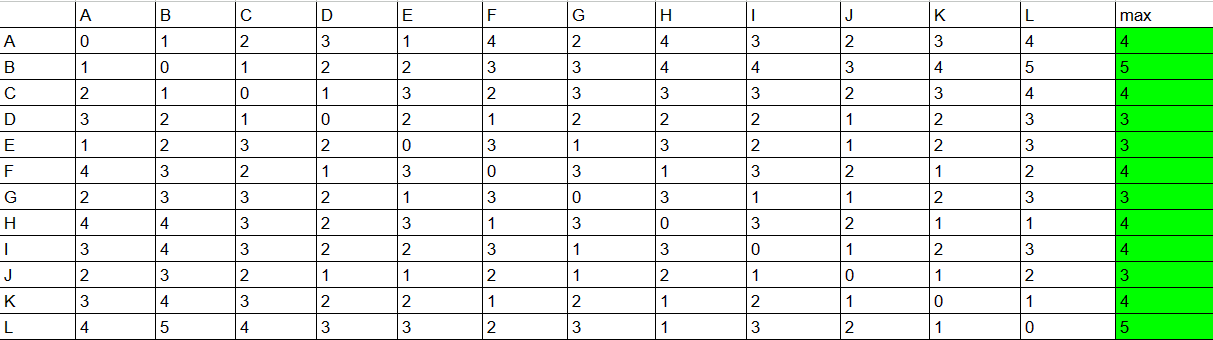
\includegraphics[width=1.1\linewidth]{pics/10ThSolution.png}
    
    Тогда \textbf{радиус} графа равен 3, \textbf{диаметр} равен 5, а \textbf{центром} могут быть вершины D, E, G или J.

\end{proof}

%%%%%%%%%%%%%% ЗАДАНИЕ №11 %%%%%%%%%%%%%%
%% Условие задания №11
\begin{problem}[11]

	Найдите хроматический многочлен данного графа:
    
    \centering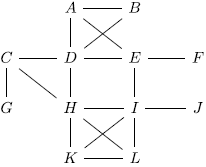
\includegraphics[width=0.4\linewidth]{pics/11ThGraph.png}
    
\end{problem}

%% Решение задания №11
\begin{proof}

    $(x-1)^{3}(x-2)(x-2)^{2}(x-3)(x-2)((x-1)^{4}-(x-1)) = (x-1)^{4}(x-2)^{4}(x-3)(x^{3}-3x^{2}+3x-1+1) = x(x-1)^{4}(x-2)^{4}(x-3)(x^{2}-3x+3)$

\end{proof}

%%%%%%%%%%%%%% ЗАДАНИЕ №12 %%%%%%%%%%%%%%
%% Условие задания №12
\begin{problem}[12]

	Из полного графа на 174 вершинах, удалили рёбра AB, AE, CH и DF. Постройте хроматический многочлен получившегося графа. Упрощать ответ не обязательно.
    
\end{problem}

%% Решение задания №12
\begin{proof}

    Ответ: $K_{174}+4K_{173}+5K_{172}+2K_{171}$ Решение приведено на следующей странице:
    
    \centering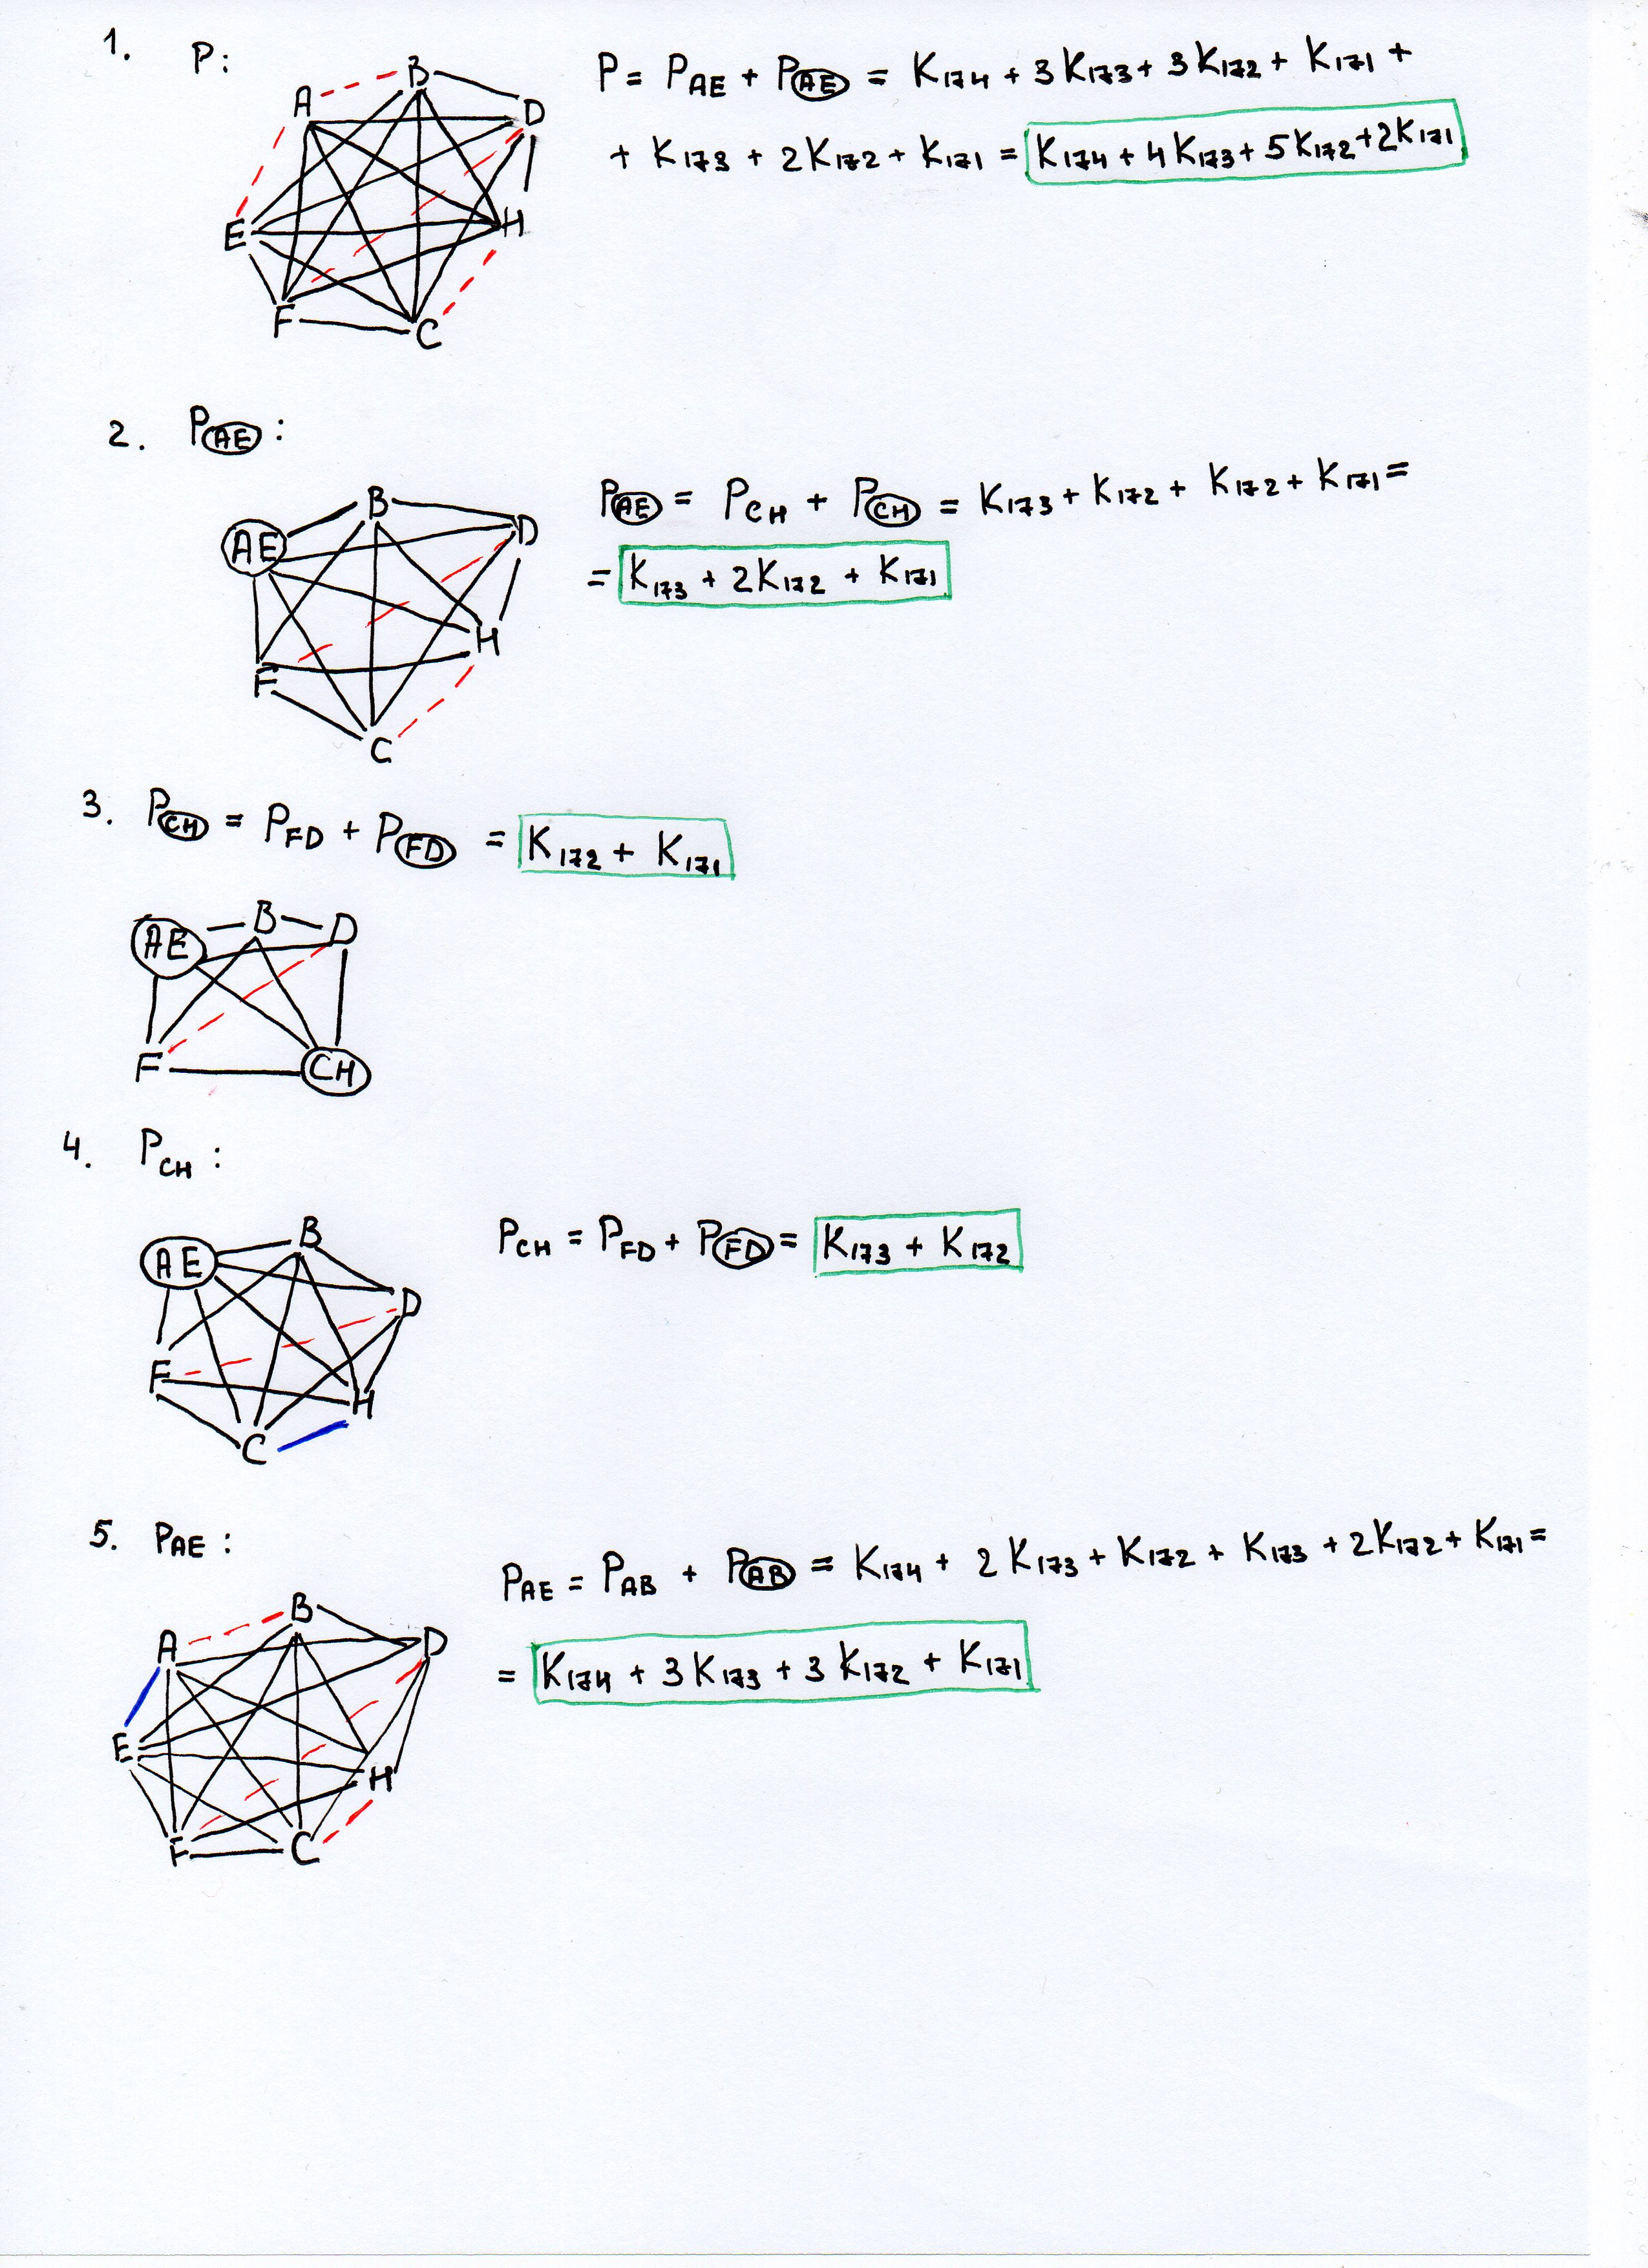
\includegraphics[width=1\linewidth]{pics/12thSolution.jpg}

    \centering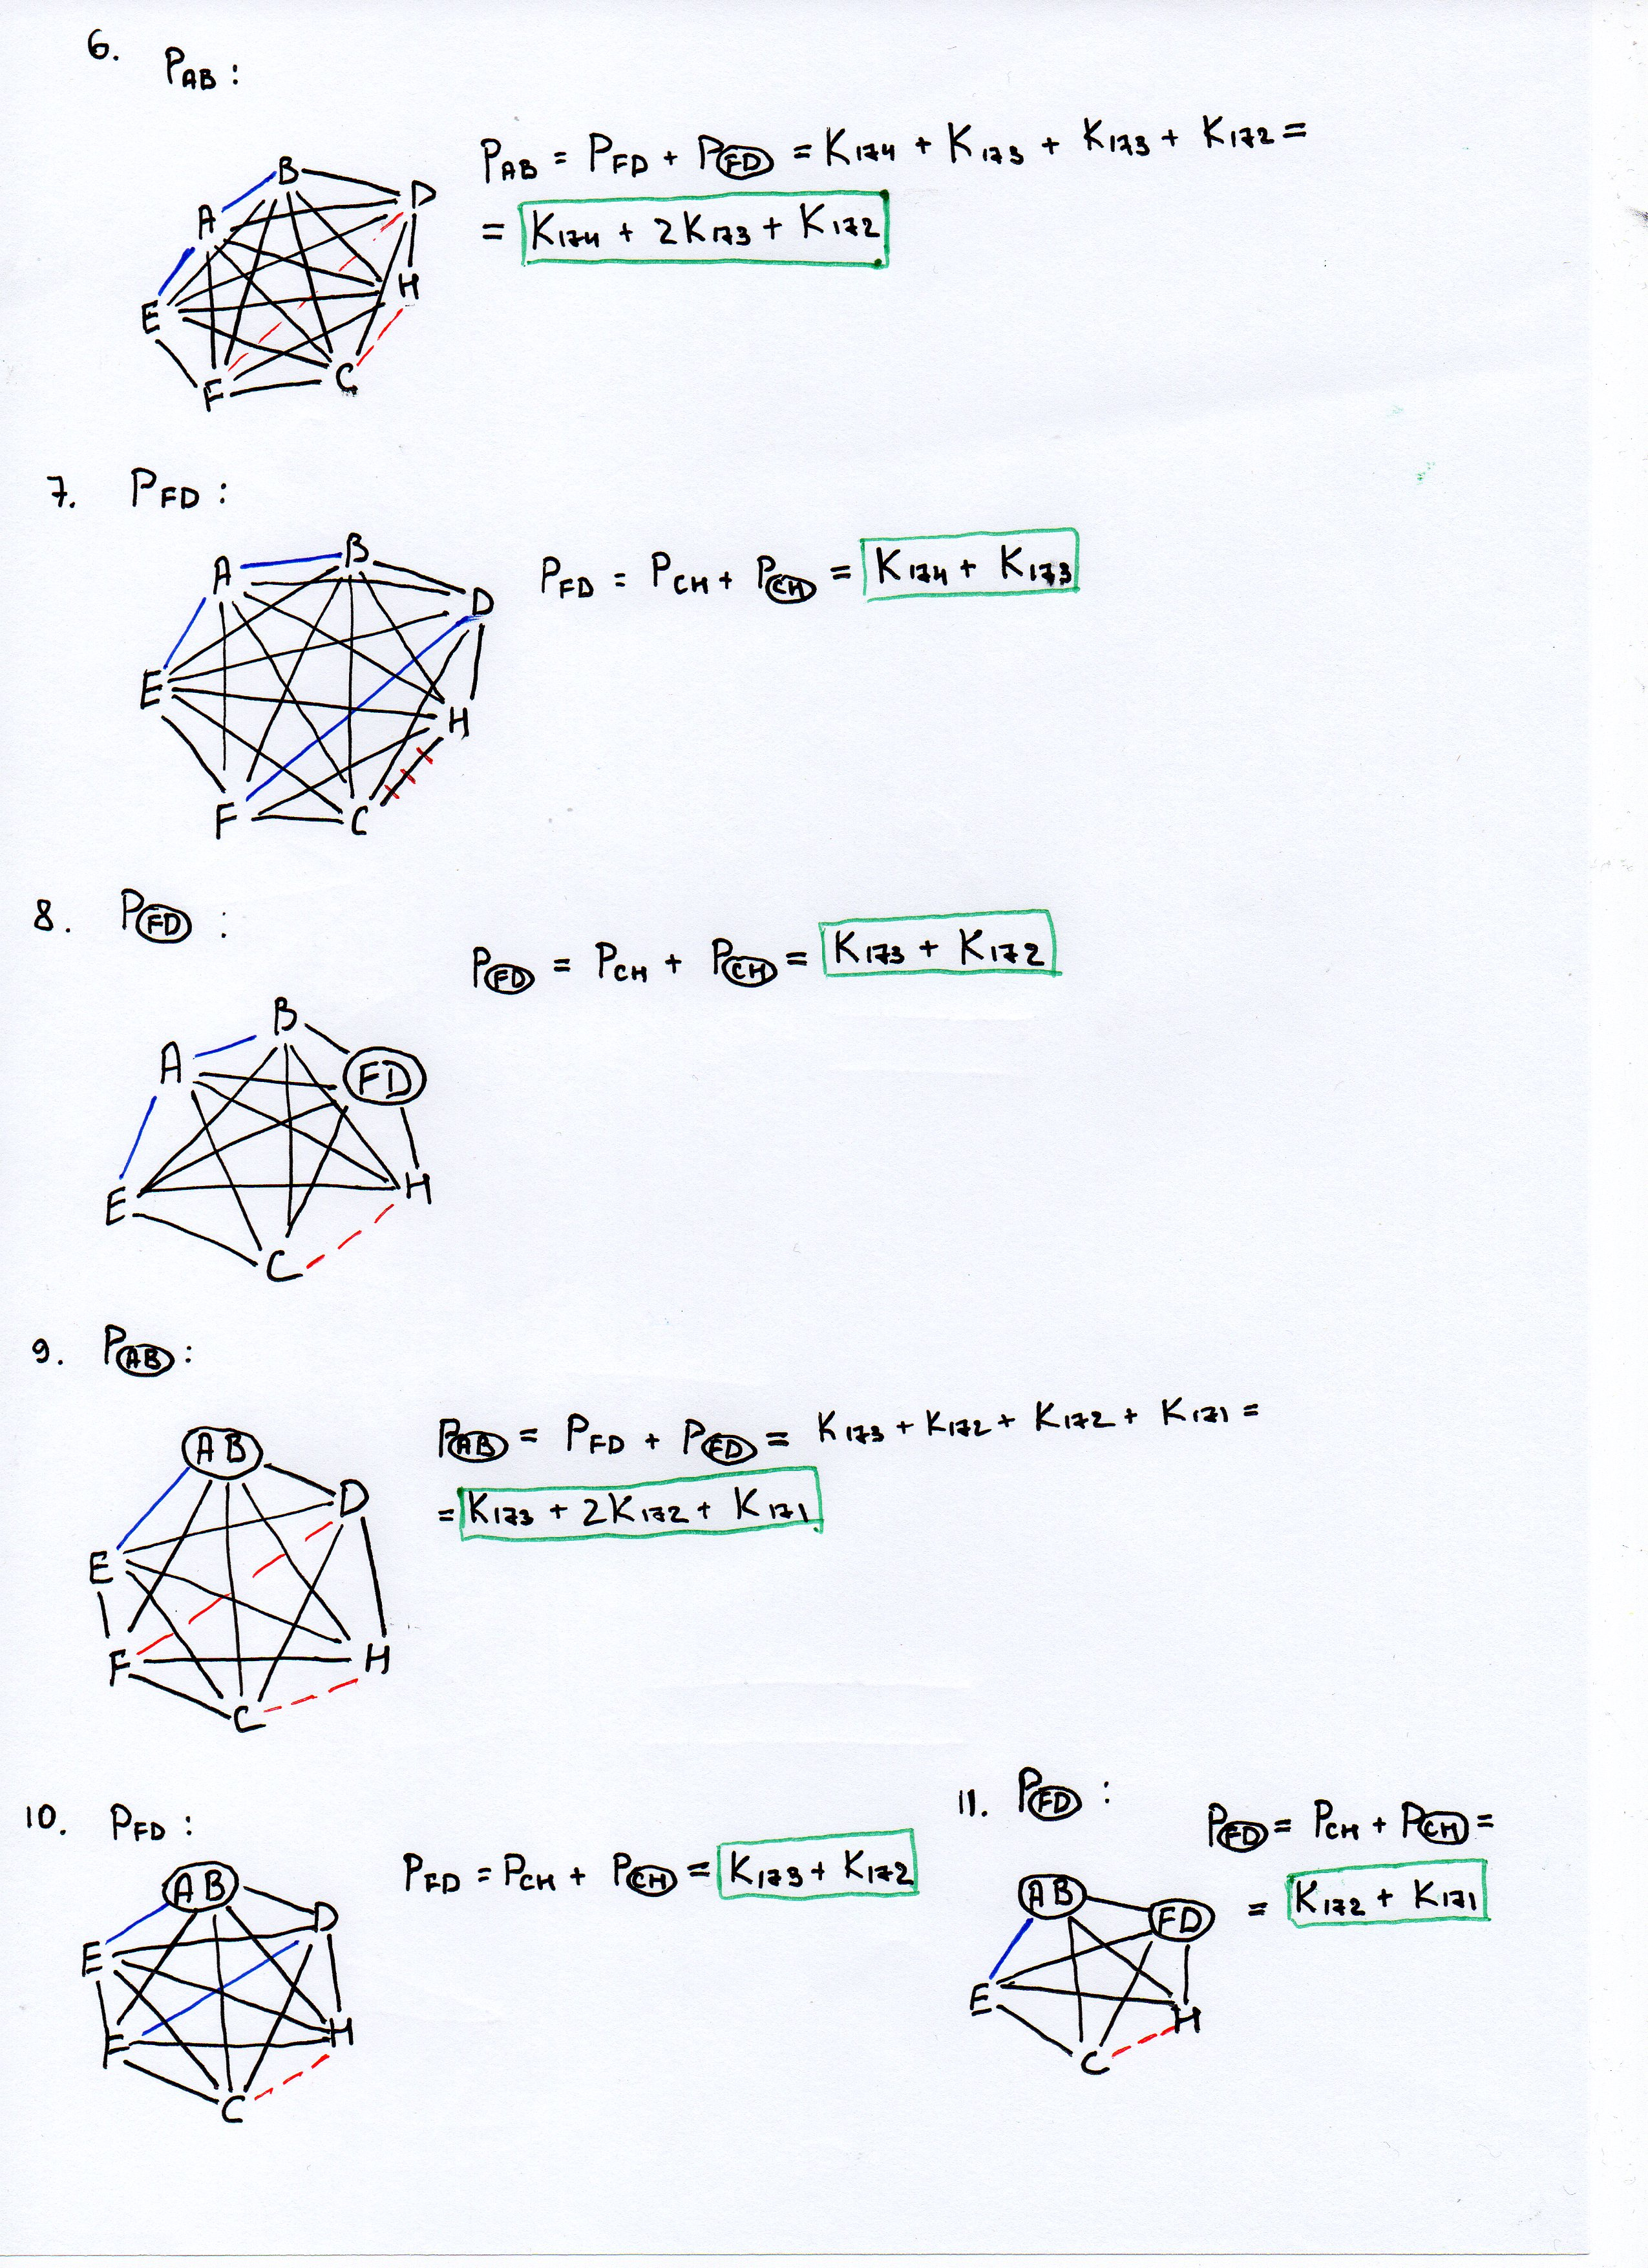
\includegraphics[width=1\linewidth]{pics/12thSolution1.jpg}

\end{proof}

%%%%%%%%%%%%%% ЗАДАНИЕ №13 %%%%%%%%%%%%%%
%% Условие задания №13
\begin{problem}[13]

	Найдите максимальный поток через данную плоскую сеть:
    
    \centering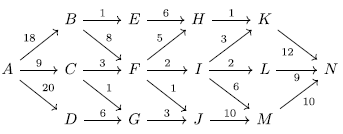
\includegraphics[width=0.5\linewidth]{pics/13thGraph.png}
    
\end{problem}

%% Решение задания №13
\begin{proof}

    Решим задачу с помощью алгоритма Форда - Фалкерсона:
    
    \begin{figure}[h]
    \centering
     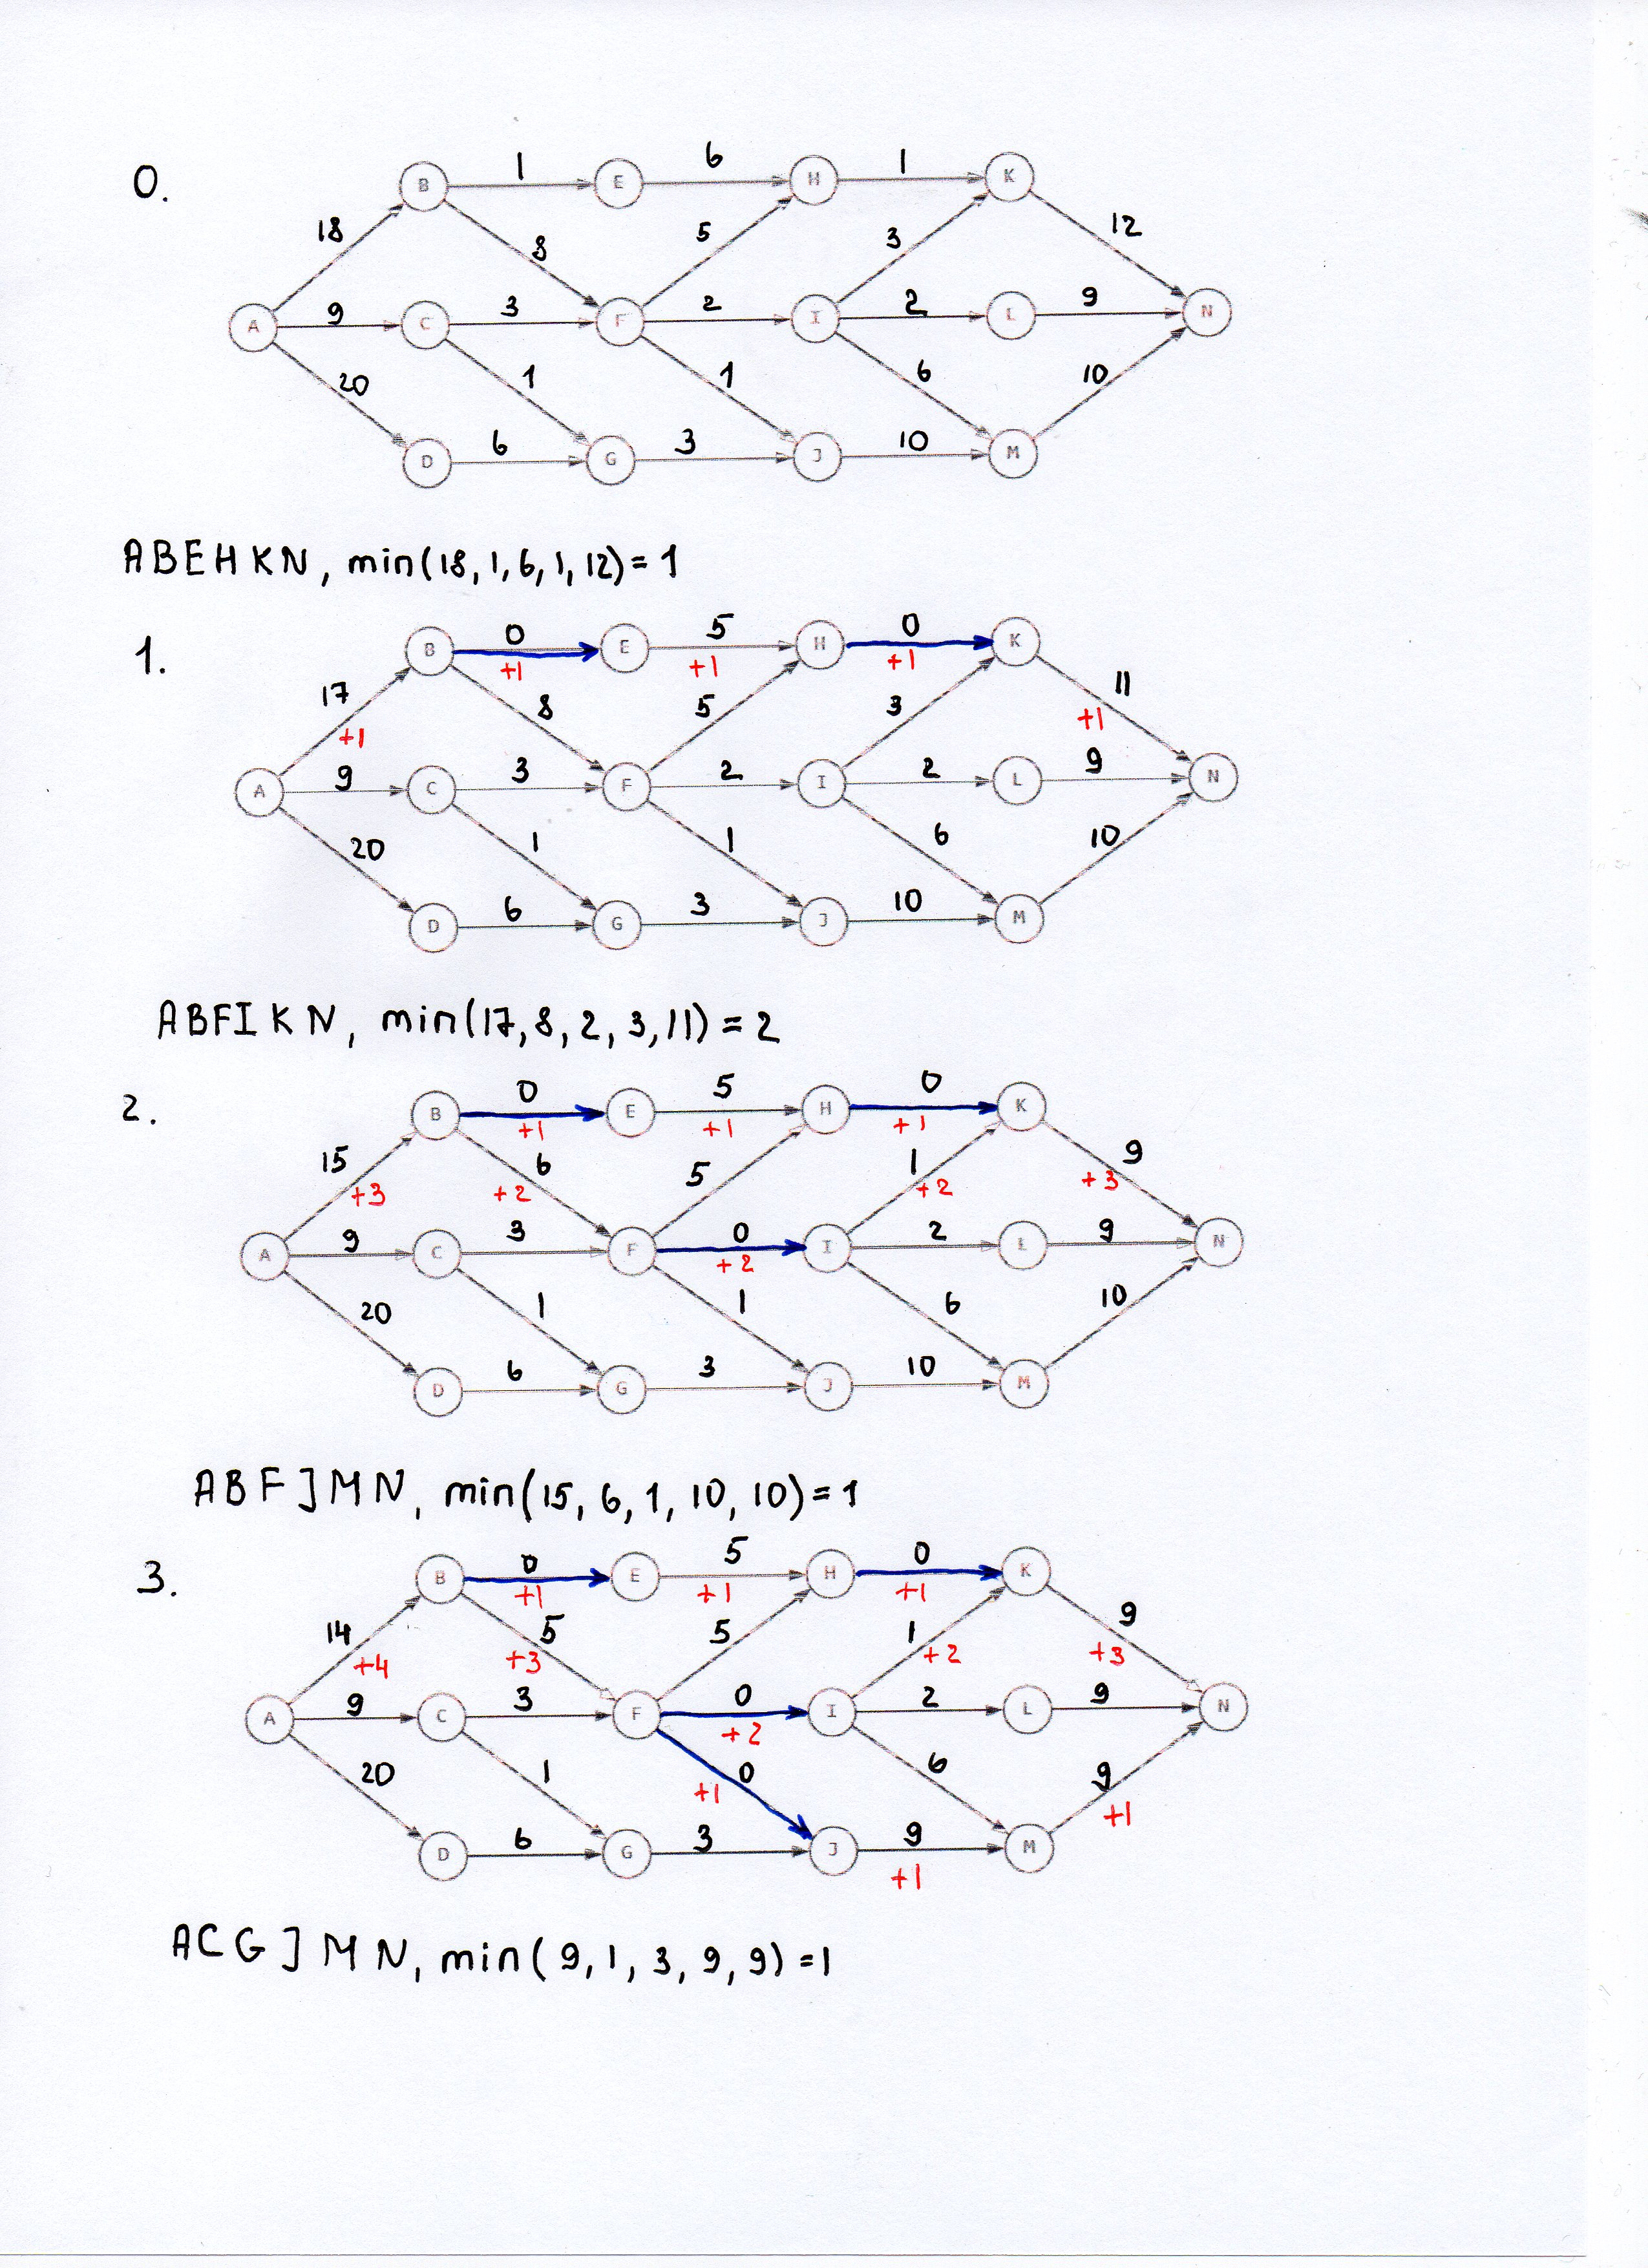
\includegraphics[width=0.7\linewidth]{pics/13thSolution1.jpg}
     \label{fig:dm}
    \end{figure}

    \begin{figure}[h]
    \centering
     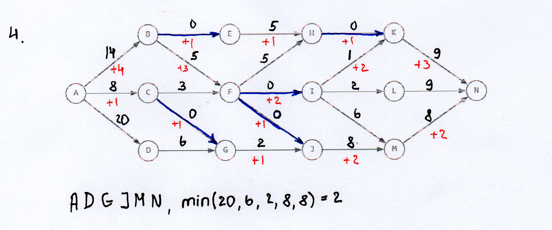
\includegraphics[width=0.65\linewidth]{pics/13thSolution4.png}
     \label{fig:dm}
    \end{figure}

    \begin{figure}[h]
    \centering
     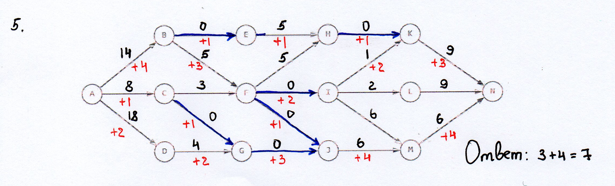
\includegraphics[width=0.65\linewidth]{pics/13thSolution5.png}
     \label{fig:dm}
    \end{figure}

\end{proof}

%%%%%%%%%%%%%% ЗАДАНИЕ №14 %%%%%%%%%%%%%%
%% Условие задания №14
\begin{problem}[14]

	Найдите максимальный поток через данную сеть:
    
    \centering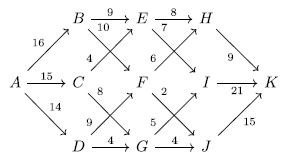
\includegraphics[width=0.55\linewidth]{pics/14thGraph.png}
    
\end{problem}

%% Решение задания №14
\begin{proof}

    Решим задачу с помощью алгоритма Форда - Фалкерсона. Решение приведено на следующей странице:
    
    \centering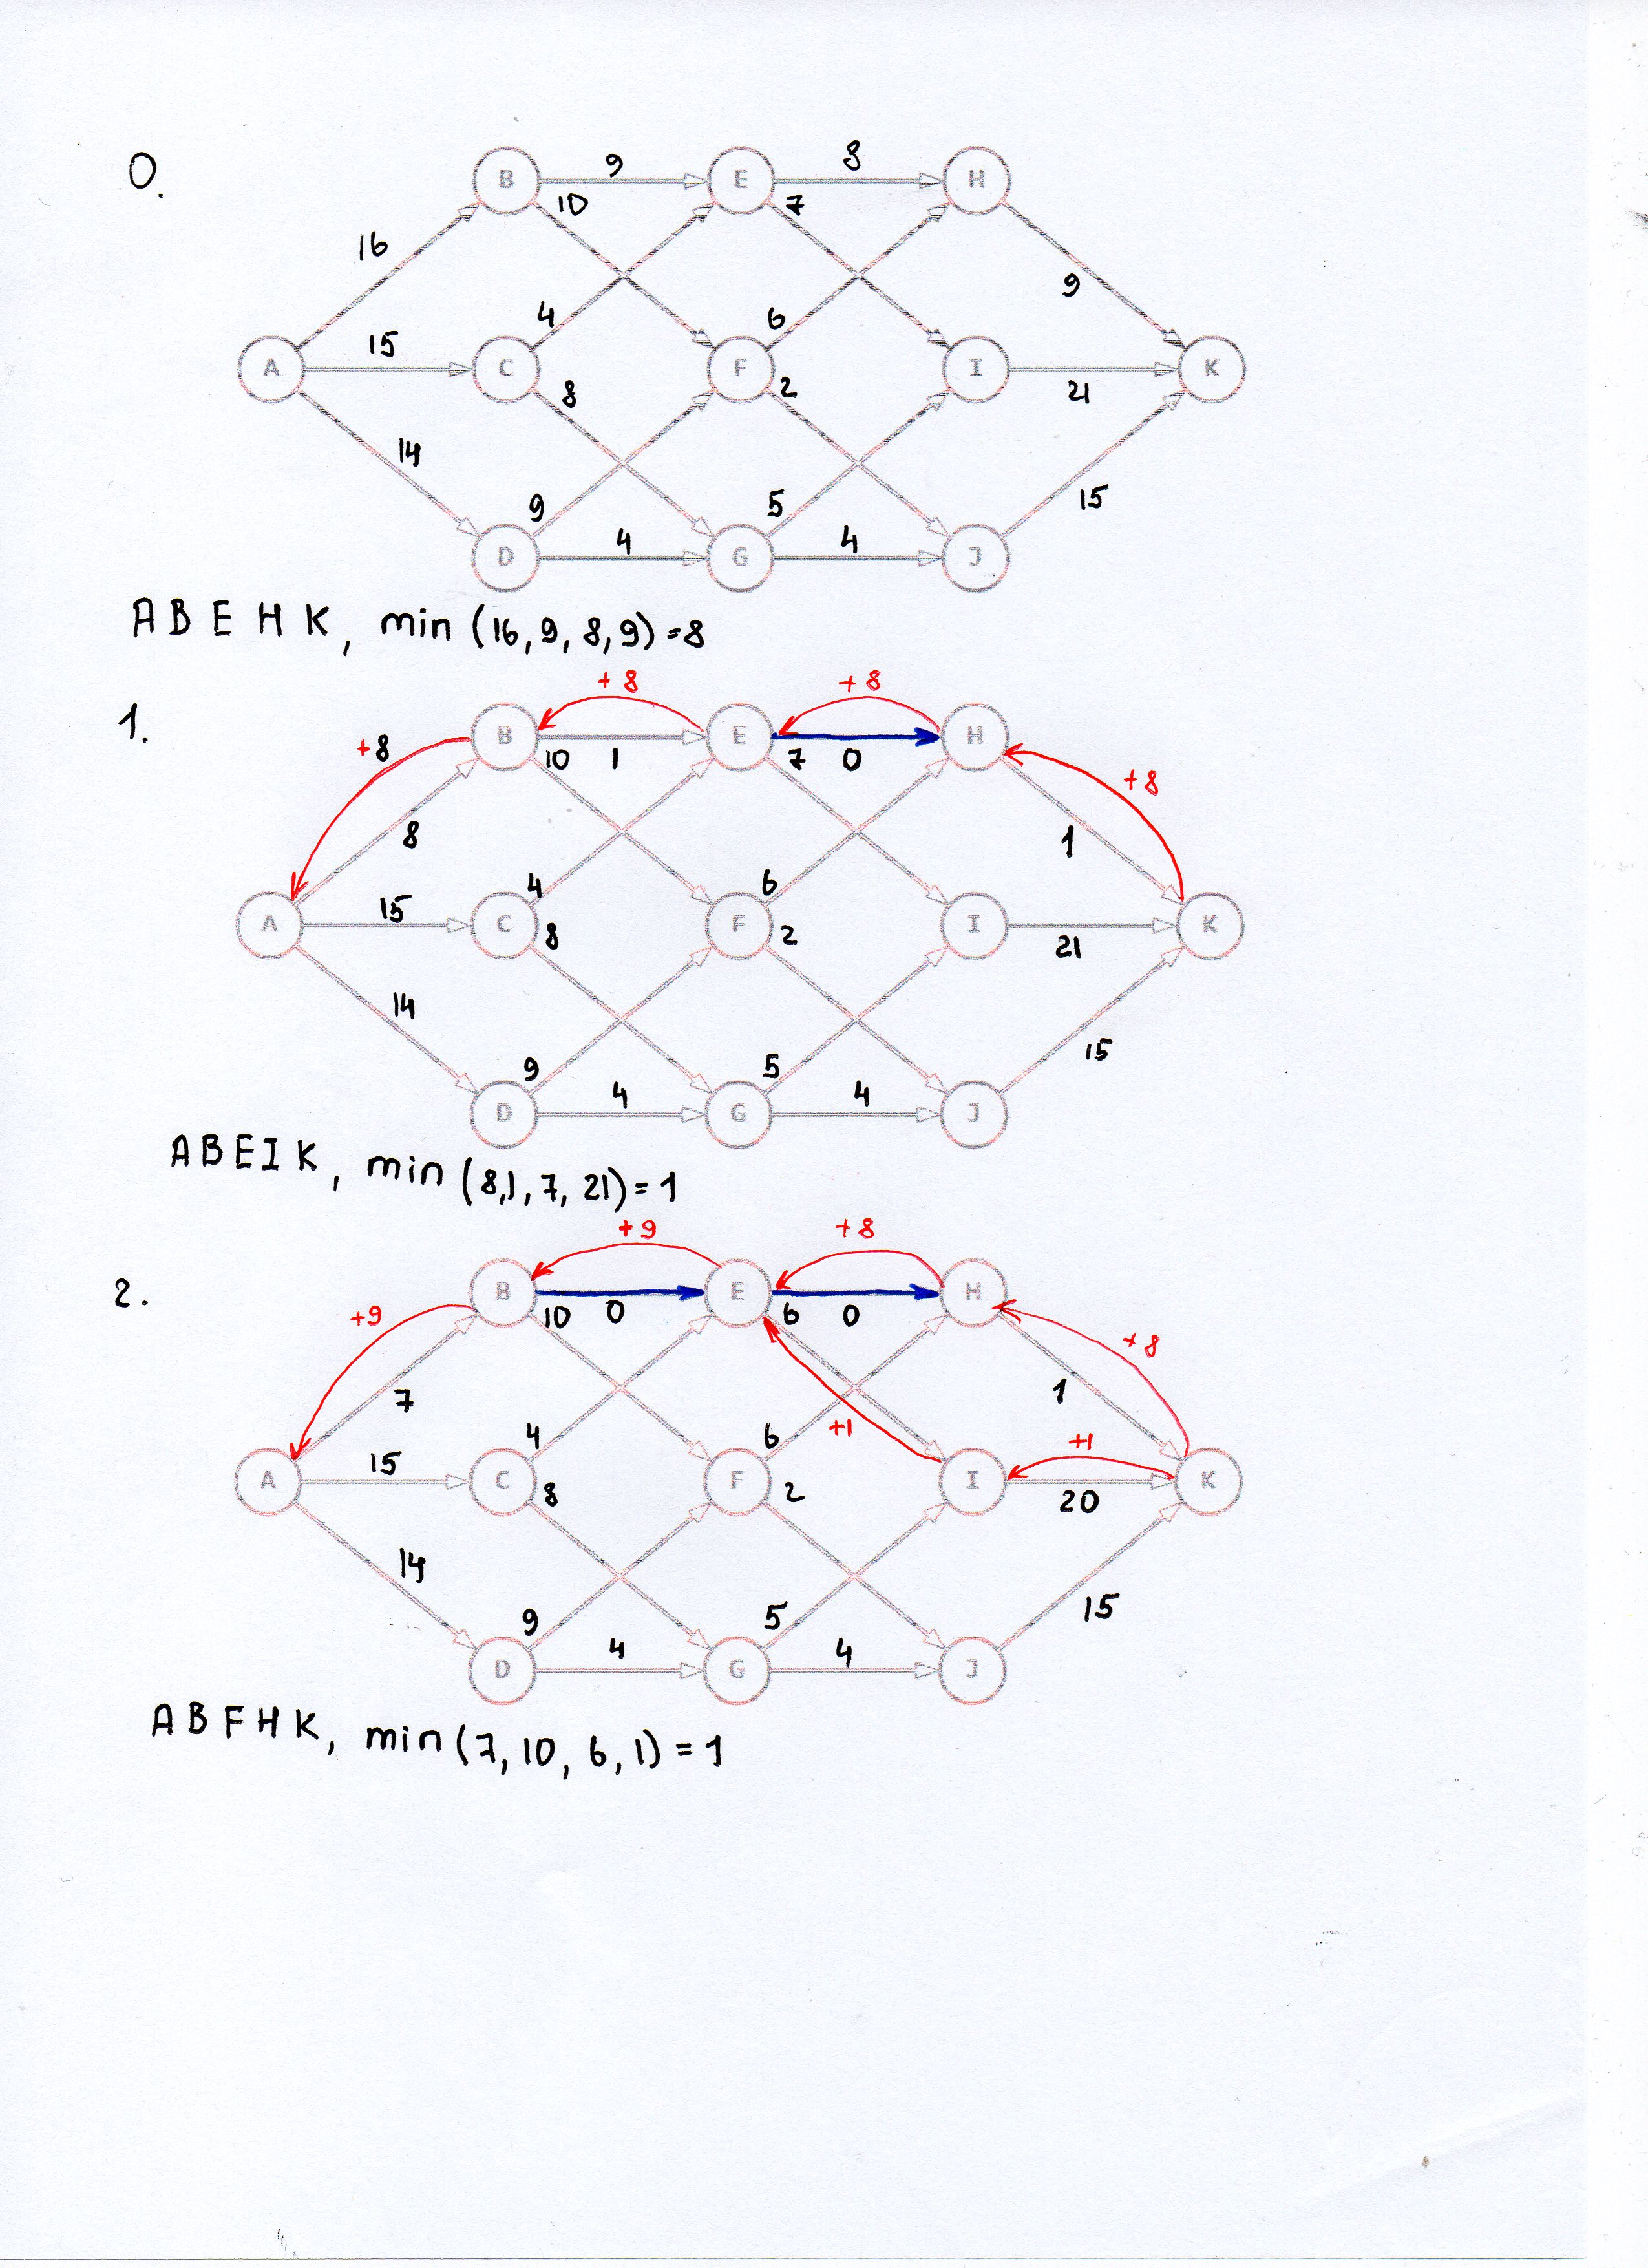
\includegraphics[width=1\linewidth]{pics/14thSolution1.jpg}

    \centering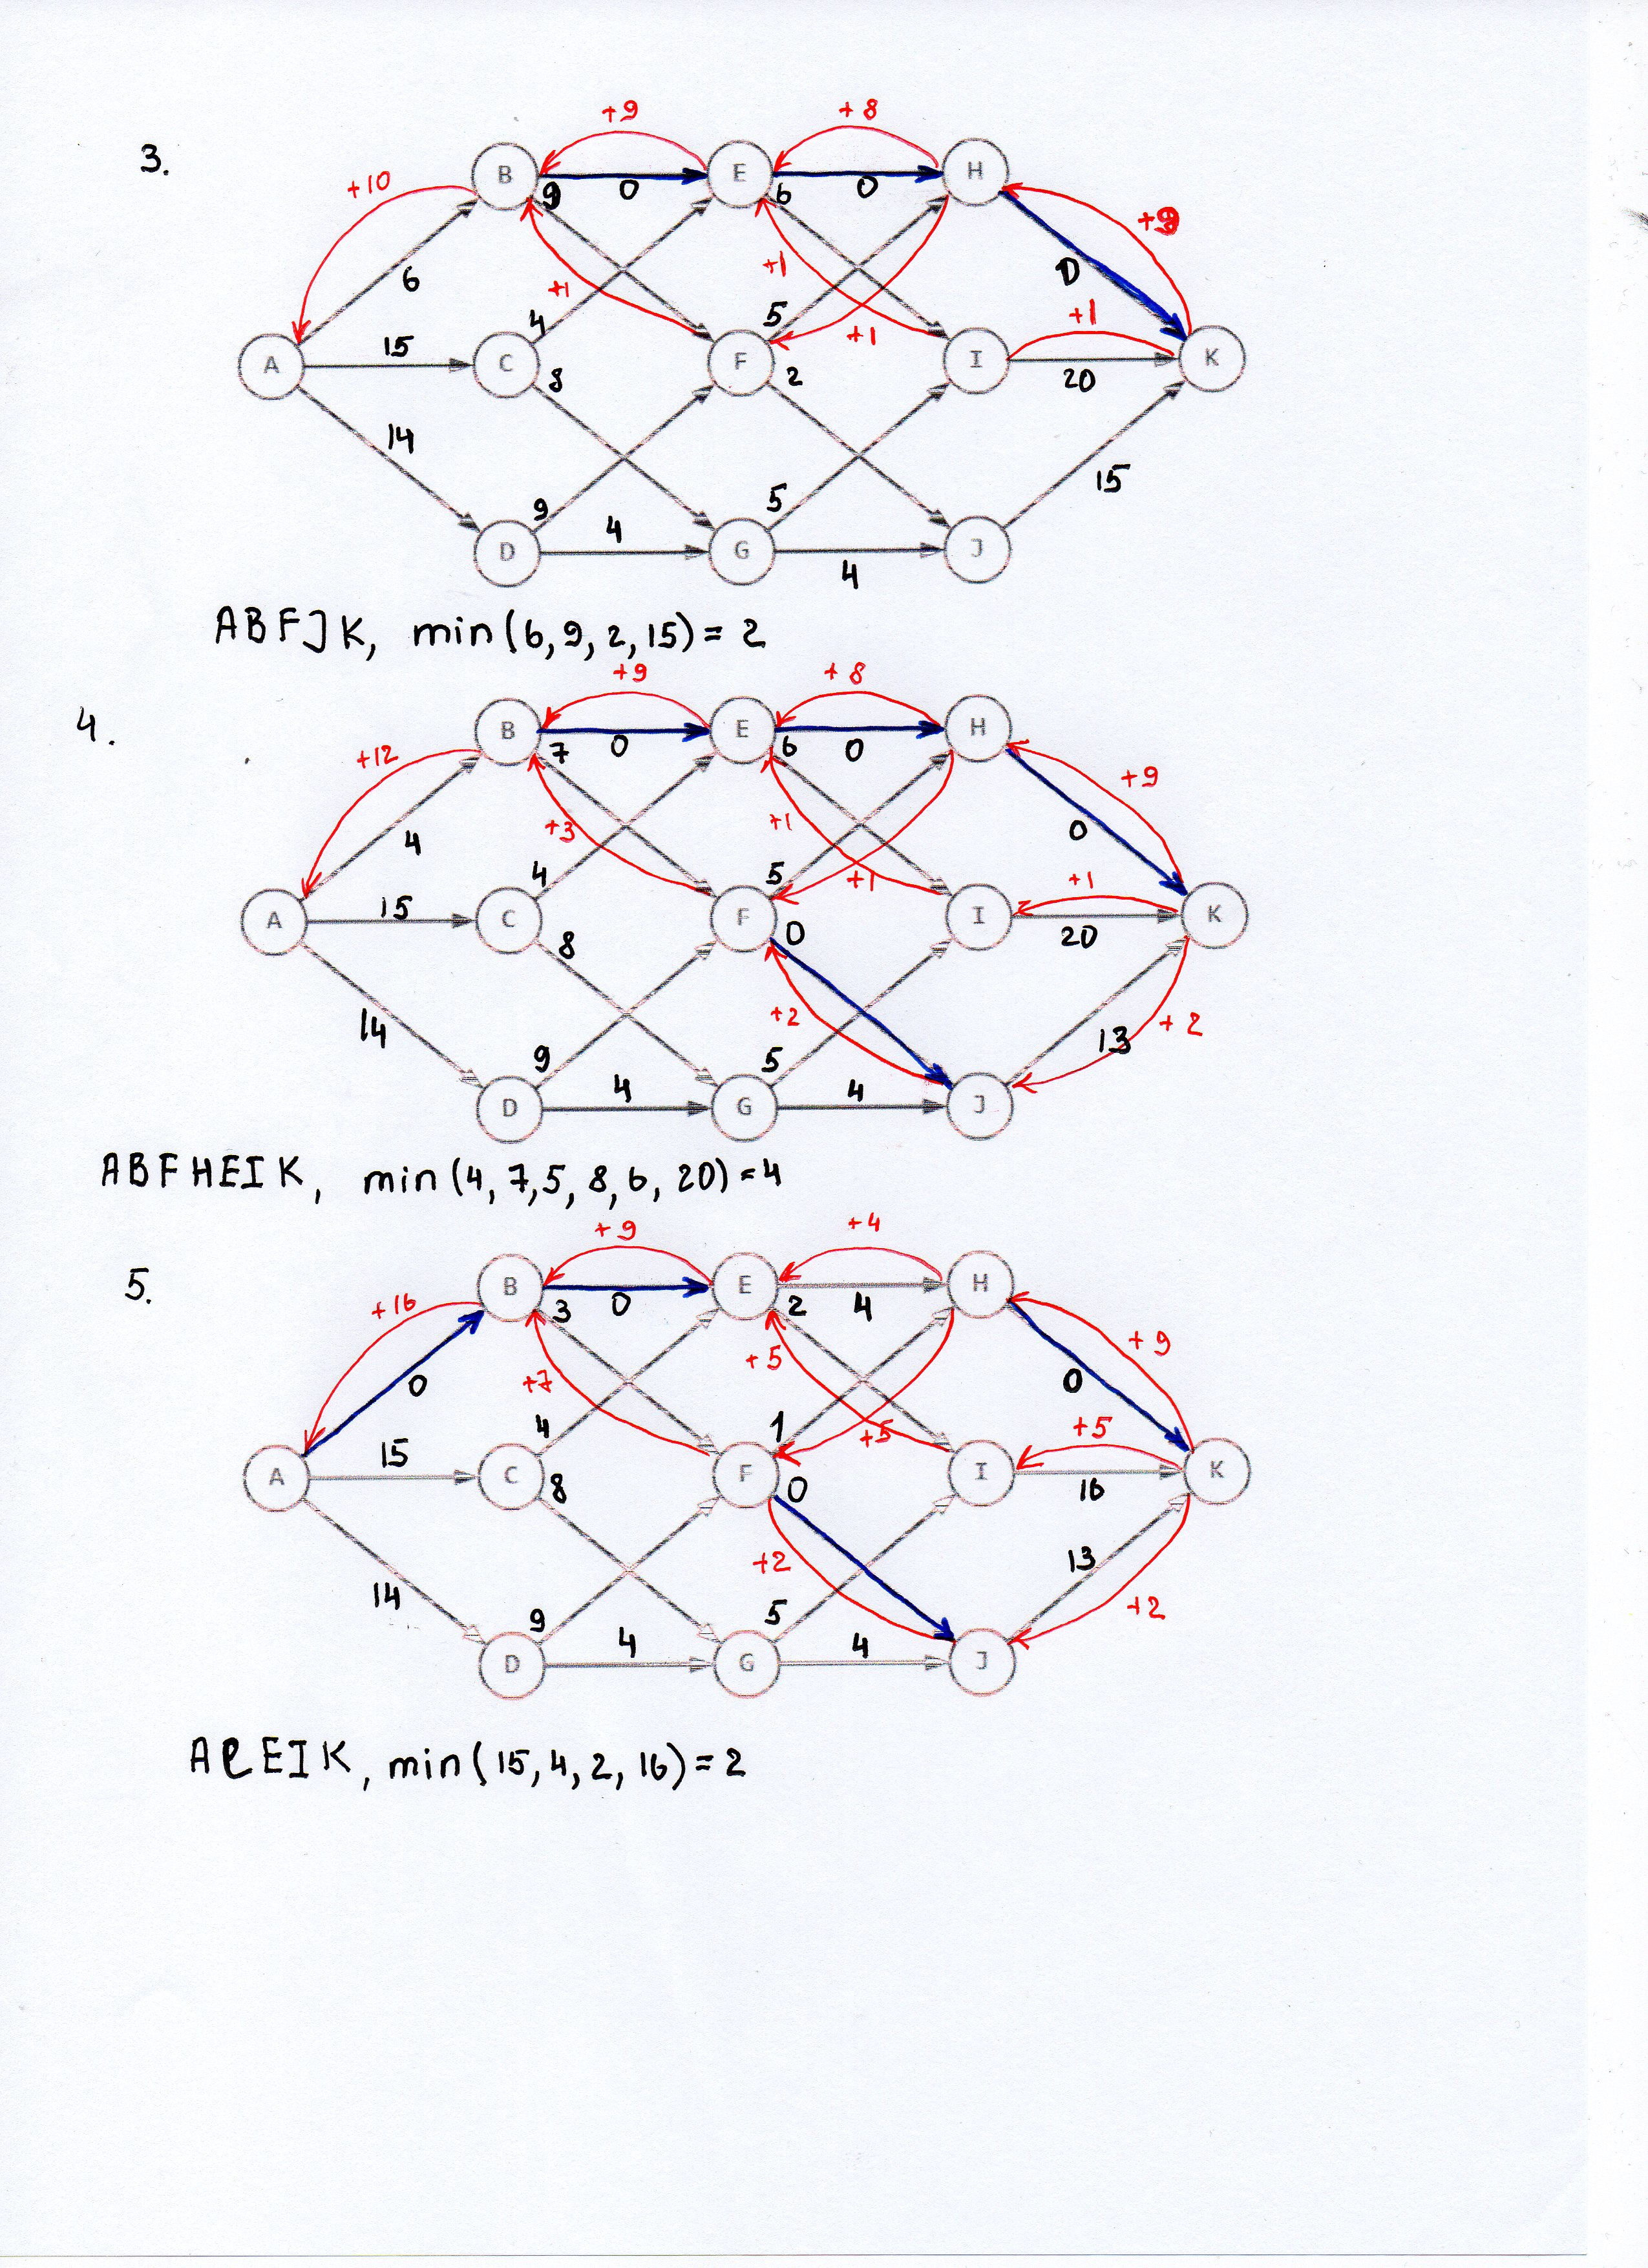
\includegraphics[width=1\linewidth]{pics/14thSolution2.jpg}

    \centering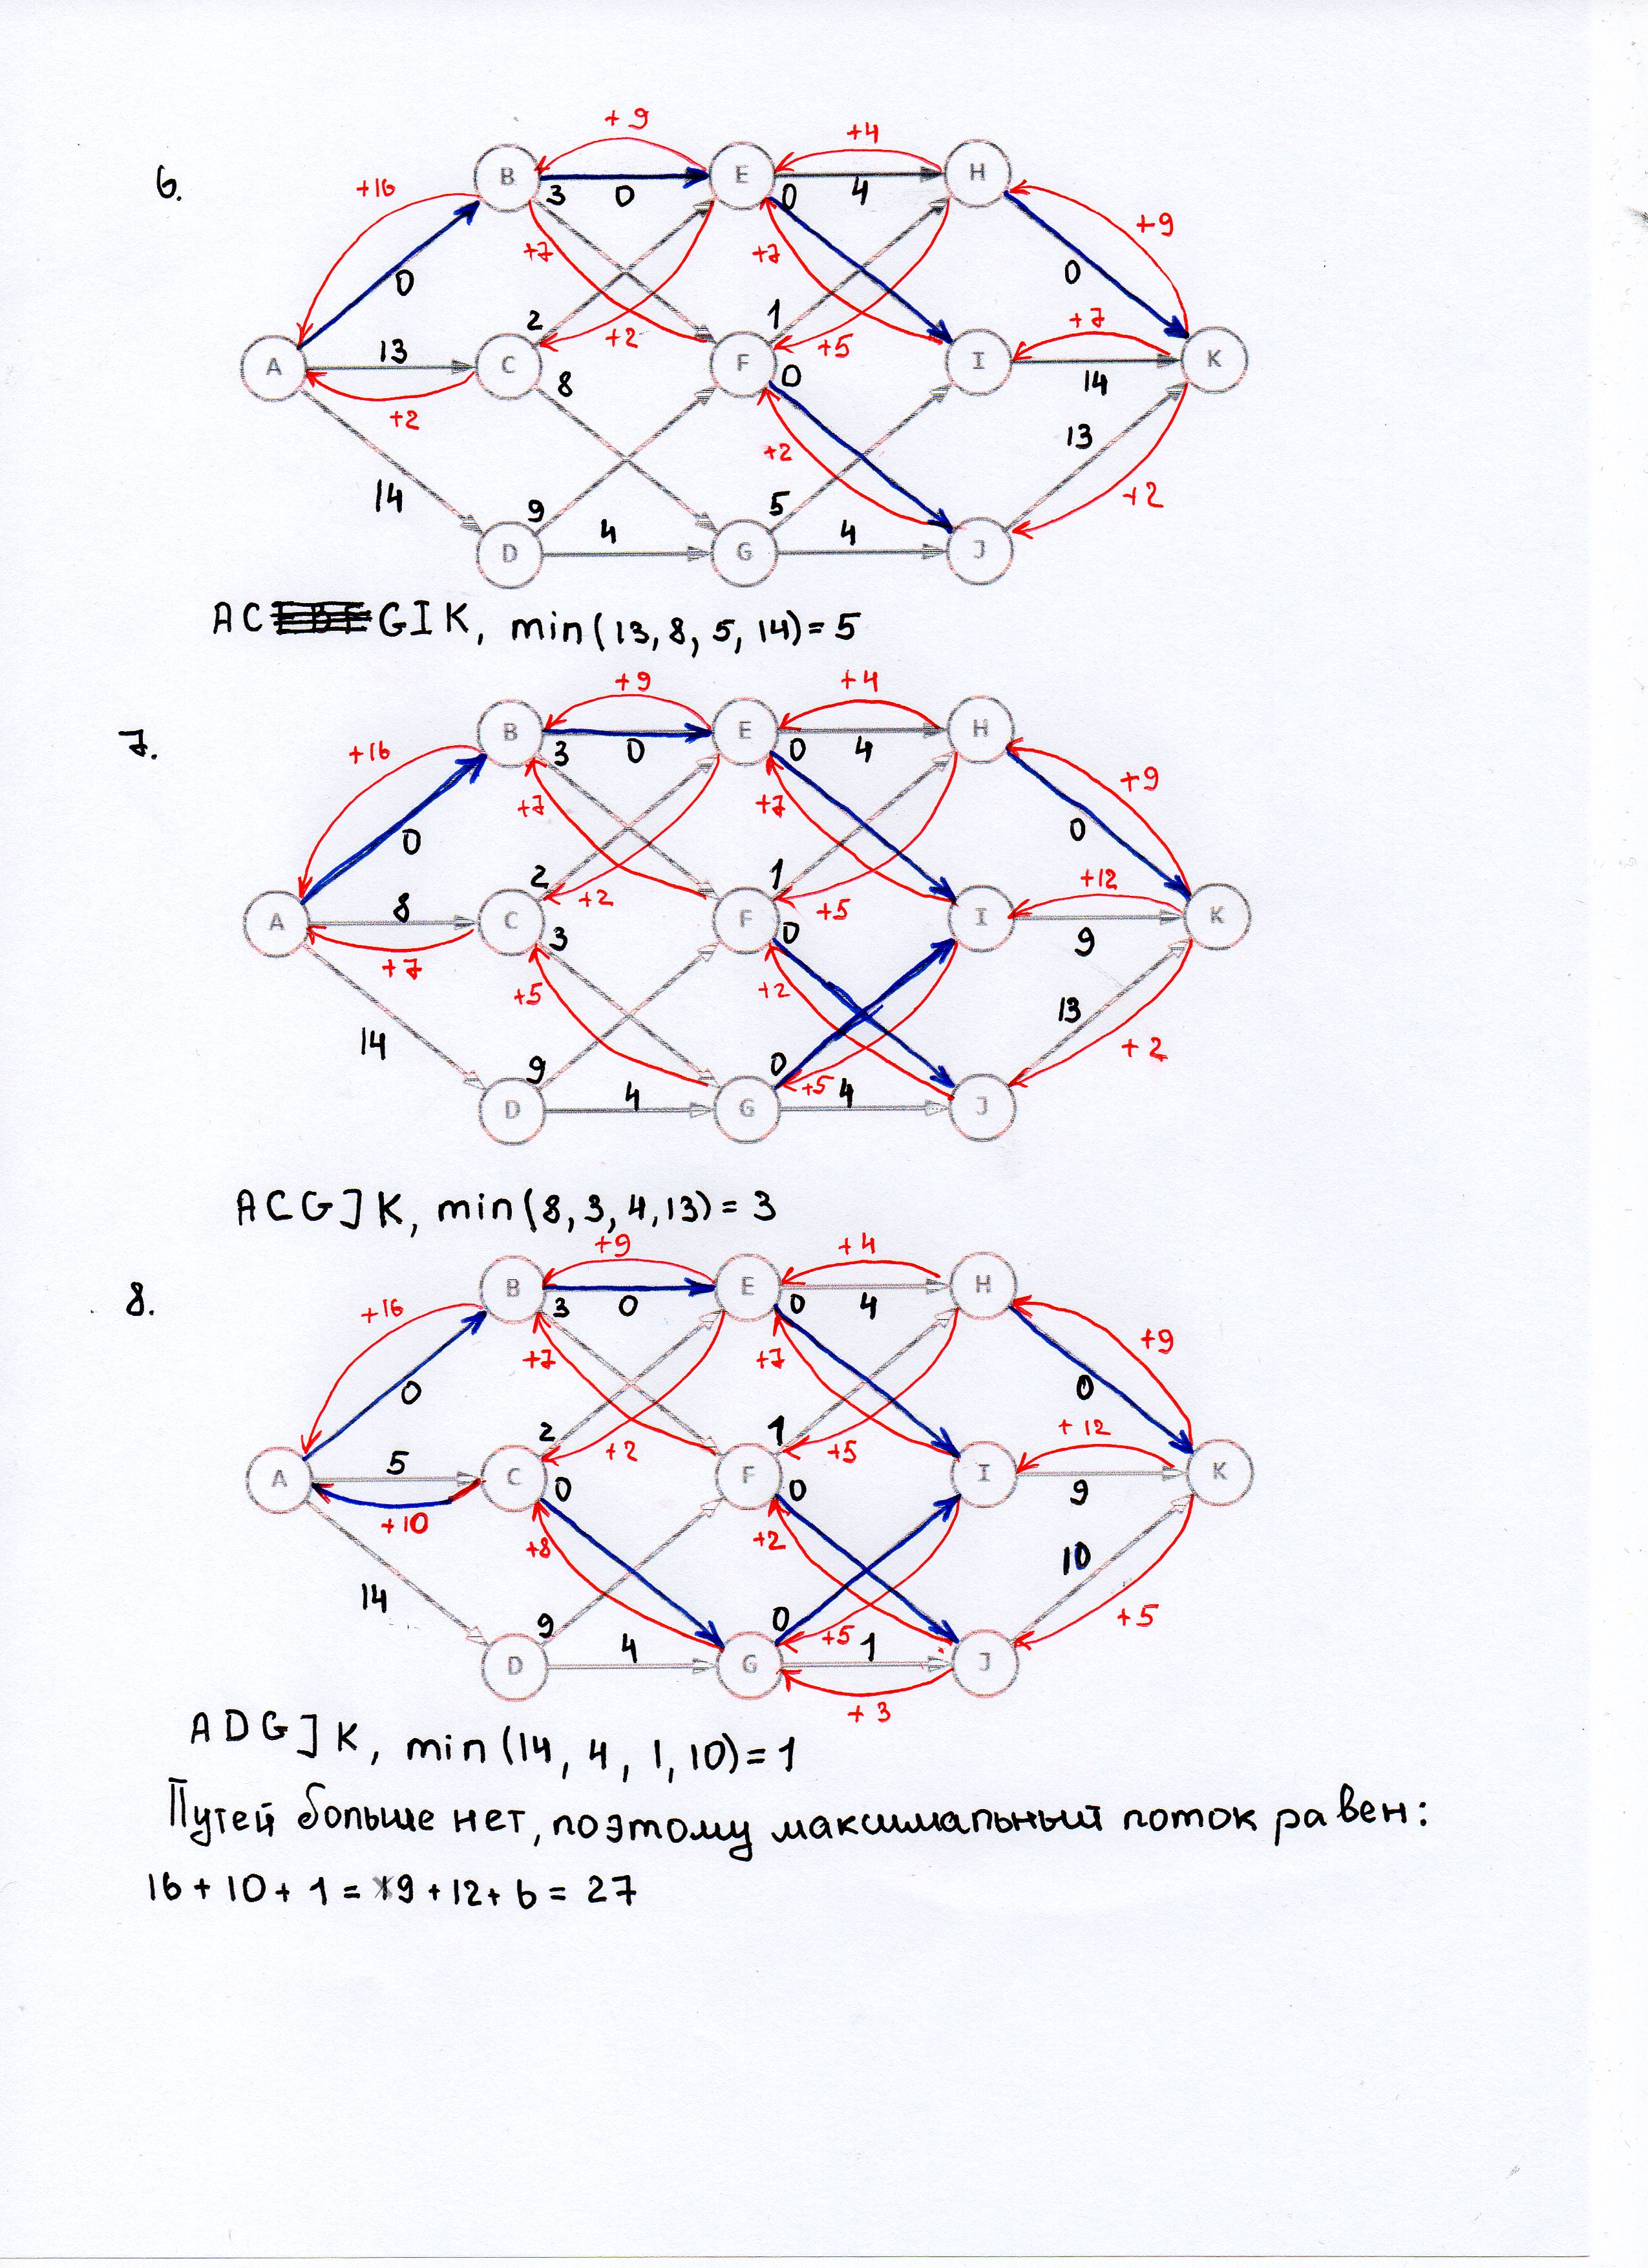
\includegraphics[width=1\linewidth]{pics/14thSolution3.jpg}

\end{proof}

%%%%%%%%%%%%%% ЗАДАНИЕ №15 %%%%%%%%%%%%%%
%% Условие задания №15
\begin{problem}[15]

	Найдите наибольшее паросочетание в двудольном графе, заданном набором рёбер:$(a,\alpha) (a,\theta) (b,\delta) (c,\beta)$ 
 
    $(c,\delta) (d,\eta) (d,\theta) (e,\epsilon) (f,\beta) (f,\gamma) (f,\delta) (f,\epsilon) (f,\zeta) (g,\beta) (g,\theta) (h,\eta)$
    
\end{problem}

%% Решение задания №15
\begin{proof}
    Построим двудольный граф:
    
    \centering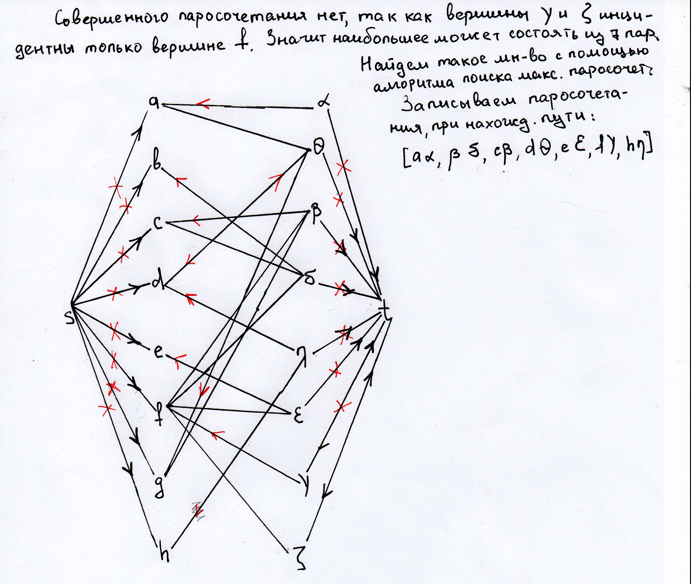
\includegraphics[width=1\linewidth]{pics/15thSolution.png}

    Ответ: [$(a\alpha) (b,\delta) (c,\beta) (d,\theta) (e,\epsilon) (f,\gamma) (h,\eta)$]
    
\end{proof}

%%%%%%%%%%%%%% ЗАДАНИЕ №16 %%%%%%%%%%%%%%
%% Условие задания №16
\begin{problem}[16]
    
    \begin{figure}[h]
    \centering
     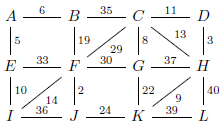
\includegraphics[width=0.35\linewidth]{pics/Graph16th.png}
     \label{fig:dm}
    \end{figure}

    б) Потсройте фундаментальную систему циклов, ассоциированную с этим деревом.

    в) Выразите через полученную фундаментальную систему цикл CGKLHGFIEFBC
    
\end{problem}

%% Решение задания №16
\begin{proof}
    
    б) По полученному остову построим фундаментальную систему циклов для рёбер в него не вошедших.

    \begin{figure}[h]
    \centering
     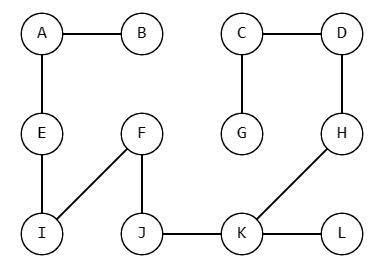
\includegraphics[width=0.4\linewidth]{pics/16th_a_solution.png}
     \label{fig:dm}
    \end{figure}

    IJ - IJFI

    EF - EFIE - $C_1$

    BF - ABFIEA - $C_2$ 

    BC - ABCDHKJFIEA- $C_3$

    FC - FCDHKJF

    FG - FGCDHKJF - $C_4$

    GH - GCDHG - $C_5$

    CH - CDHC

    KG - KGCDHK - $C_6$

    HL - HLKH - $C_7$

    в) Красным отмечены рёбра принадлежащие данному циклу, но отсутствующие в остове. Синим отмечен весь данный цикл.

    \begin{figure}[h]
    \centering
     \includegraphics[width=0.4\linewidth]{pics/16th_с.png}
     \label{fig:dm}
    \end{figure}

    По ранее построенной систем, выражаем данный цикл (у каждого непринадлежащего ребра остову есть фундаментальный цикл).
    
    $CGKLHGFIEFBC = Z$
    
    $Z = C_1\bigoplus C_2\bigoplus C_3\bigoplus C_4\bigoplus C_5\bigoplus C_6\bigoplus C_7$
    
\end{proof}